\section{Planlægning}
Der blev fra projektets start udarbejdet en tidsplan.
Gennem hele forløbet har der sideløbende været fokus på både udvikling og rapport/dokumentations skrivning.
Gruppen ønskede ikke at lave enten udvikling eller rapport. Sideløbende med udvikling af systemet, blev der skrevet dokumentation tilhørende dette område. Der skulle også skrives afsnit til rapporten inden man var færdig med opgaven. \\
Dette har betydet at alt dokumentationen er skrevet mens der blev udviklet det var i frisk erindring.
Projektet har derfor haft milepæle, som skulle overholdes, for ikke at bruge for lang tid på dokumenter i forhold til udvikling. Disse kan ses på figur \ref{fig:Tidsplan}

\begin{figure} [H]
	\begin{center}
		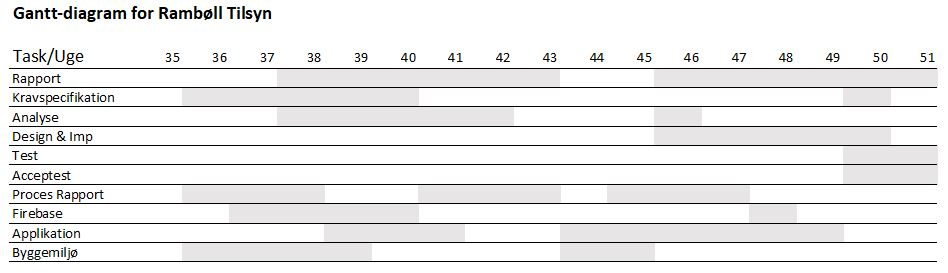
\includegraphics[height=10cm, width=16cm]{Planlaegning/Tidsplan}
	\end{center}
	\caption{Tidsplan for projektet.}
	\label{fig:Tidsplan}
\end{figure}

\clearpage

